\chapter{Analog amplifiers}
One of the goals of the thesis is to automate the design of analog amplifiers which are electronic circuits that are used to amplify the input signal.

\section{Common Emitter Amplifier} \label{ce-amp}

\begin{figure}[H]
    \centering
    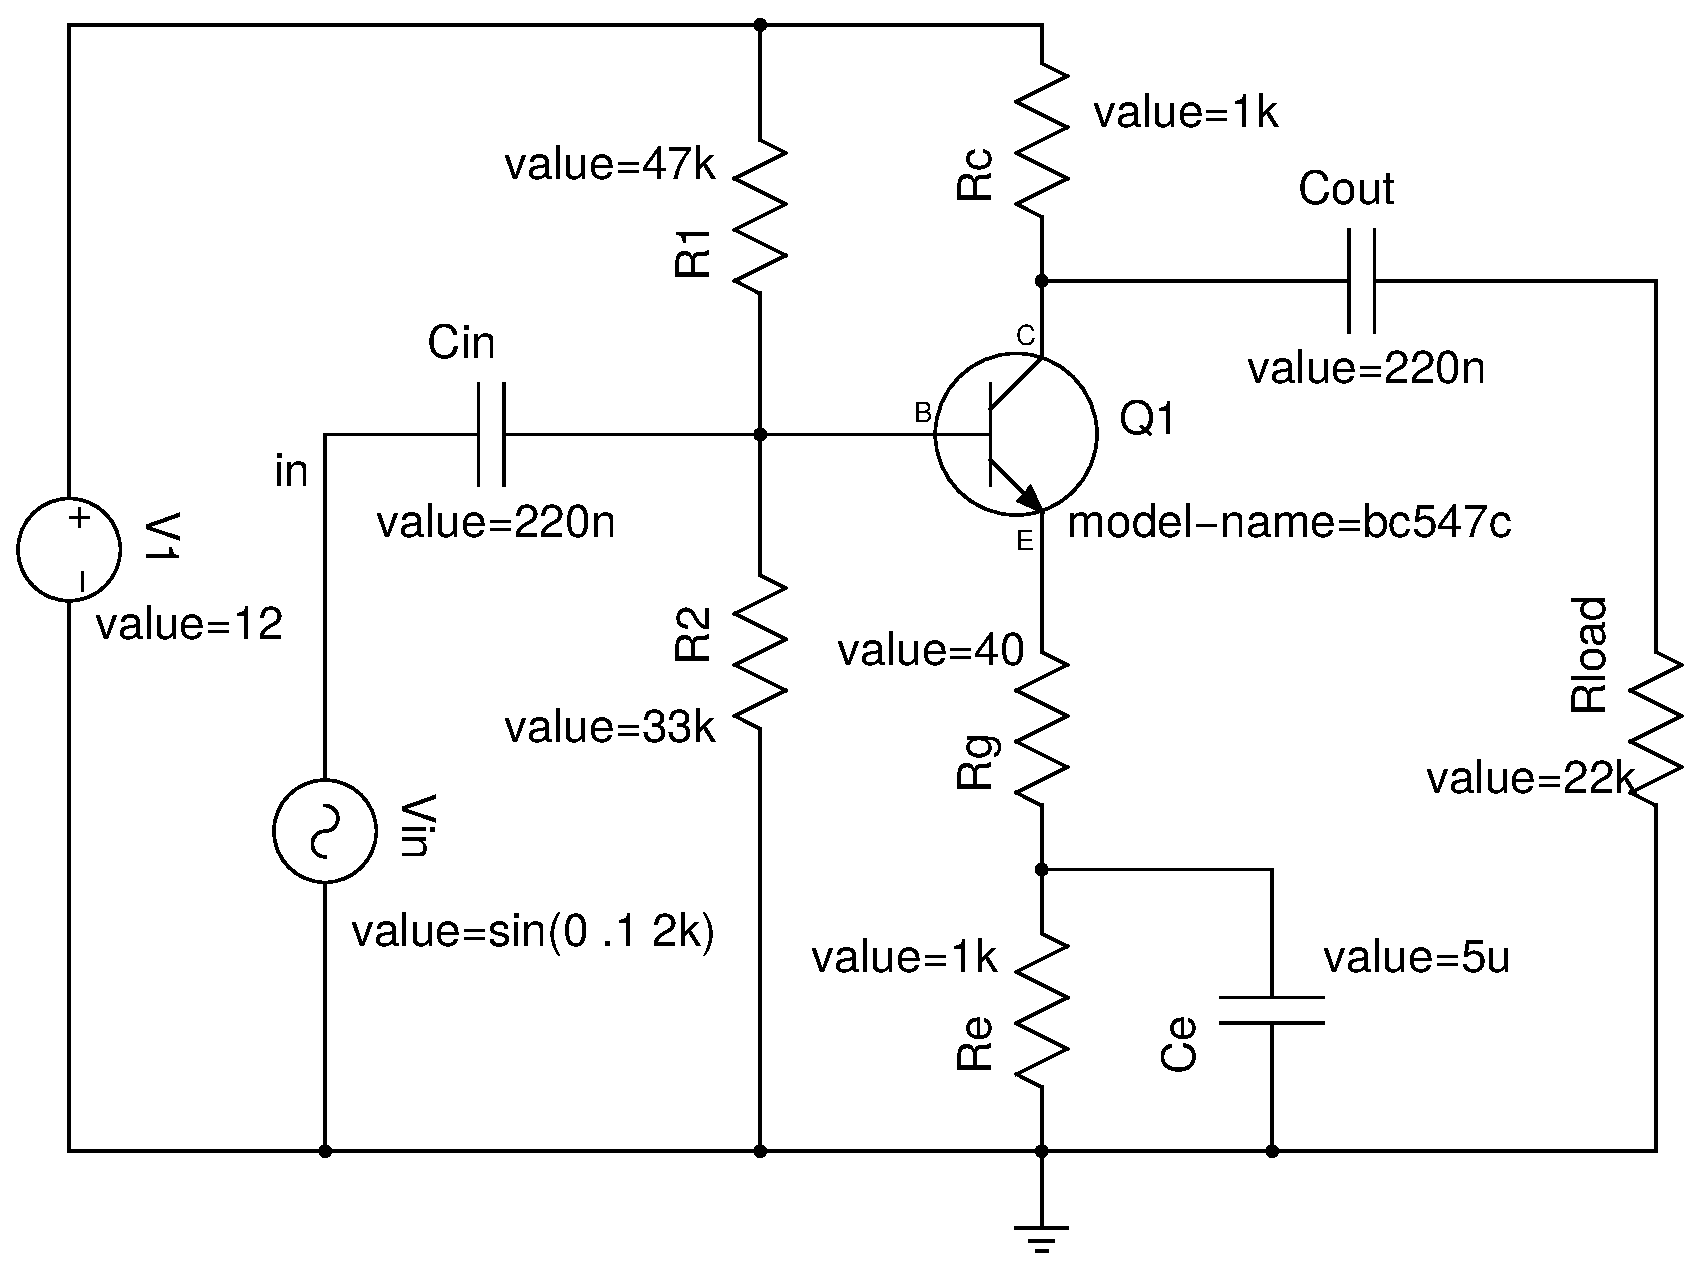
\includegraphics[scale=0.45]{ce-amplifier}\label{ce-amplifier}
    \caption{Circuit diagram for the common emitter amplifier}
\end{figure}

The subject of the optimization are elements $R1$, $R2$, $Rc$, $Rg$, $Rc$, $Cin$, $Ce$. These elements represent the solution variables in the evolutionl and make up the vector $\vec{x}$ which is thoroughly discussed in section \ref{mutation-section}.

\section{ngSPICE}
ngSPICE is an open-source circuit simulator based on SPICE (\textit{Simulation Program with Integrated Circuit Emphasis}). It uses a language which syntax has been inherited from SPICE for describing circuits.\\
An example of such description of the circuit from section \ref{ce-amp} is shown in listing \ref{ce-amp-lst}. The first line contains the name of the circuit and on the next four lines, there is a description of the transistor used in the circuit. On the next lines, there is a list of the circuit's elements. The name of the element is on the first position followed by the numbers or names of the nodes which the element is connected to. The last position contains the properties of the element. The second last line contains the description of the simulation. In this case, we do a transient analysis of the circuit for \SI{1.22}{\milli\second} with the sampling period \SI{20}{\micro\second}. This netlist can be generated by using the gEDA toolkit which is also an open-source project.

\begin{lstlisting}[caption={description of an amplifier using the SPICE syntax},
                   label={ce-amp-lst},
                   captionpos=b,
                   numbers=left]
 amplifier
.model bc547c NPN (BF=730 NE=1.4 ISE=29.5F IKF=80M IS=60F
       + VAF=25 ikr=12m BR=10 NC=2 VAR=10 RB=280 RE=1 RC=40
       + VJE=.48 tr=.3u tf=.5n cje=12p vje=.48 mje=.5
       + cjc=6p vjc=.7 mjc=.33 isc=47.6p kf=2f)
Vin in 0 sin(0 .1 2k)
V1 4 0 9
Ce 0 5 5u
Cout 1 out 220n
Cin in 3 220n
Rc 1 4 1k
Rload 0 out 22k
Re 0 5 1k
Rg 5 2 40
R2 0 3 33k
R1 3 4 47k
Q1 1 3 2 bc547c
.TRAN 20u 1.22m
.end
\end{lstlisting}

The last version of ngSPICE contains a C API which makes the simulator the ideal choice for utilizing it with the evolutionary algorithms. Every chromosome (candidate solution) in the evolution represents one amplifier and the simulator is used to determine the quality of it. In figure \ref{ce-amplifier-sim} we can see the simulation output of the circuit from listing \ref{ce-amp-lst} which is the same circuit as in section \ref{ce-amp}. This circuit was also built using real electronic components in order to verify the simulation results. The measurement results of the real circuit proved that the simulation works correctly for this circuit as the values corresponded to each other.\\
The API is used to pass the description of the amplifier to the simulator, run the simulation and obtain the simulation results. The results are in the form of arrays in C which represent time and the corresponding voltage values. These arrays have equal length which depends on the simulation duration and the sampling period. The default input frequency for the amplifier is \SI{2}{\kilo\hertz}. The duration of the simulation is set to \SI{1.22}{\milli\second} and it contains approximately two and a half period of the output signal. The duration does not need to be longer because the shape of the waveform does not change afterwards. The sampling period is \SI{20}{\micro\second}. The array containing the output voltage is used for the evaluation of the chromosomes which is thouroughly discussed in section \ref{chromosomes-evaluation}.\\
The simulator is launched several thousand times during a typical evolution and it takes most of the computation time. During the implementation of the algorithms discussed in section \ref{evolution-strategies} and the integration of the simulator, it emerged that there are memory leaks on several places in the source code of the simulator. This was a problem as the simulator leaked memory in every iteration. A significant amount of time was spent on fixing these bugs and the result is that the memory leaks have been removed. These improvements were proposed to the development team and they are currently waiting for their approval, so that they can be incorporated into the new version of ngSPICE.

\begin{figure}[H]
    \centering
    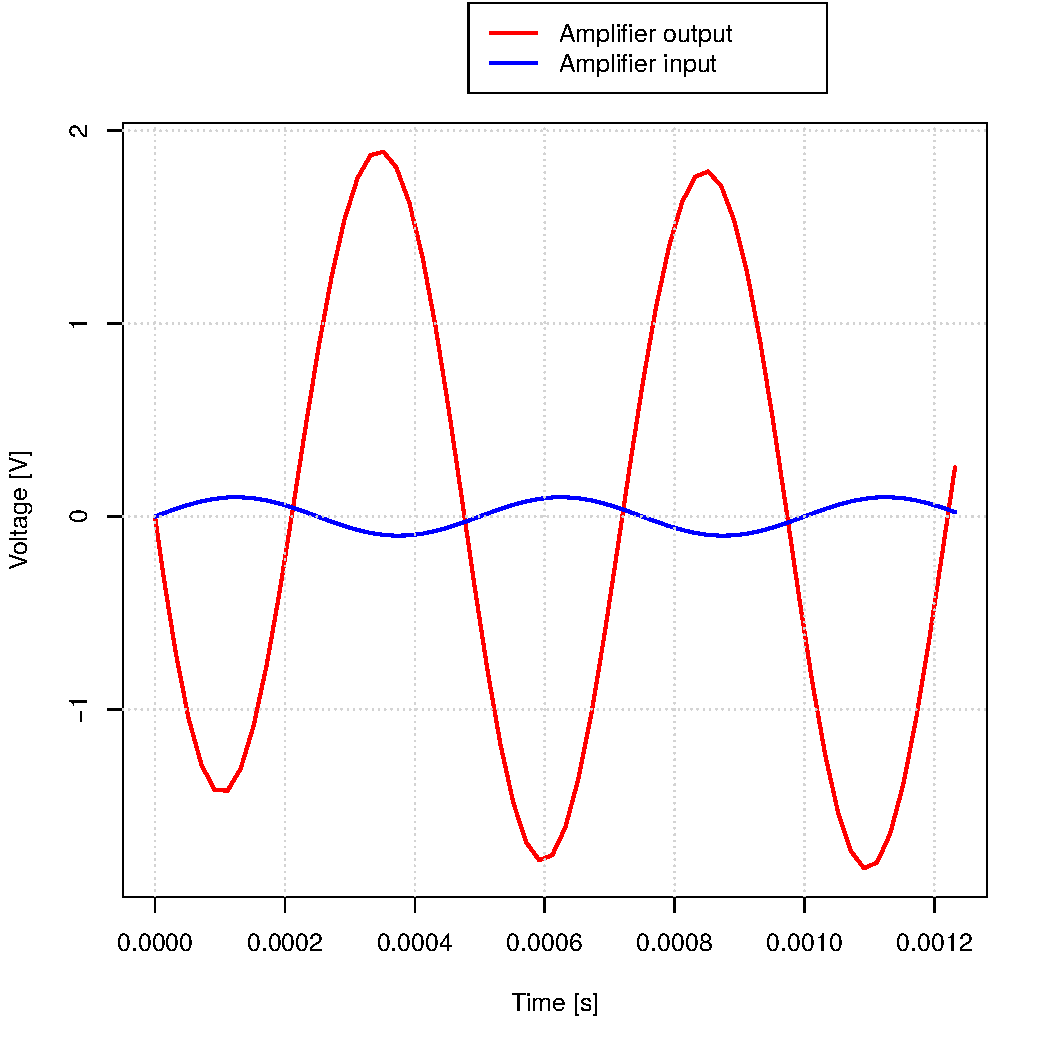
\includegraphics[scale=.7]{ce-amplifier-sim}\label{ce-amplifier-sim}
    \caption{Simulation of the common emitter amplifier}
\end{figure}
